\section{Ambiente da pesquisa}
\label{ambiente}
 Esta Seção apresenta o ambiente elaborado para verificar a validade da DSL de Cotas em relação aos objetivos da presente pesquisa. Desse modo, são descritos os critérios utilizados para definir os grupos de usuários convidados, os critérios de avaliação da \gls{API} implementada para classificar e aprovar os candidatos, e também apresentar o questionário aplicado com os participantes.
 
\subsection{Metodologia de avaliação da DSL}
\label{metododsl}

 Segundo \citeonline{kateMoran2018}, estudos qualitativos de usabilidade tentam compreender o pensamento e as dificuldades vivenciadas pelos indivíduos, geralmente este tipo de estudo apresenta aos usuários atividades abertas que têm o potencial de expor problemas na interface do sistema. 
 
 \citeonline{kateMoran2018} também cita alguns princípios básicos para elaboração de tarefas para qualquer tipo de teste com usuário, tais como:
 
 \begin{enumerate}
    \item[a)] Atente-se ao que seus usuários precisam fazer com o seu produto para inspirar suas tarefas;
    \item[b)] Evite fornecer dicas para a sua tarefa. Não descreva os passos exatos que o usuário precisa fazer, deixe que eles descubram por si mesmos;
    \item[c)] Sempre faça um teste piloto para as tarefas, isso é essencial para evitar obter acidentalmente dados incorretos ou ruins.
    
\end{enumerate}
 
 Considerando essas orientações foi realizado um teste piloto da \gls{DSL} em Abril de 2020. Para tanto, foi instalado o software \textit{TeamViewer} para acesso remoto a uma máquina virtual \textit{Linux} contendo a ferramenta \gls{MPS}, no qual a DSL foi disponibilizada para teste. Todavia, observou-se que a ferramenta de acesso remoto dificultava o uso da linguagem, no sentido de apresentar lentidão durante a execução dos comandos. Outro problema percebido foi a falta de instruções sobre o uso da linguagem, bem como foram encontradas dificuldades de visualização de alguns elementos, tendo em vista que a fonte fornecida era pequena.
 
 A partir dessa avaliação foram feitas as correções necessárias, por meio da troca da ferramenta de acesso remoto para o software \textit{VNCViewer} e a elaboração de um documento para subsidiar os usuários. Desse modo, foi elaborado um manual de utilização da DSL (APÊNDICE X), no qual foram apresentados os objetivos e os elementos da linguagem, os principais comandos para edição das regras de negócio e o link para o vídeo explicativo também elaborado pelo autor, no qual se exibiu um exemplo de uso das principais funcionalidades. O ambiente para avaliação da DSL pode ser observado na Figura \ref{ambiente}.
 
 
  \begin{figure}[ht!]
\centering

\caption{\textmd{Ambiente de avaliação no \gls{MPS}}}
\label{fig:ambiente}
\fcolorbox{gray}{white}{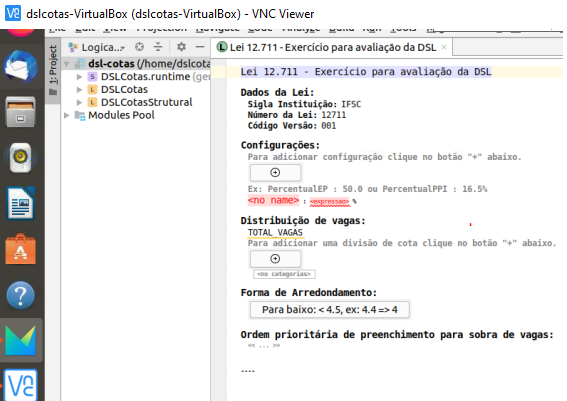
\includegraphics[width=0.76\textwidth]{chapters/metodologia/imagens/ambienteimg.png}}

\par\medskip\textbf{Fonte:} Elaboração do autor (2020) \par\medskip

\end{figure}


 
 No que concerne à seleção dos usuários para os testes, baseando-se em \citeonline{nielsen2012many}, entre os meses de Abril e Maio de 2020 buscou-se 20 pessoas com perfis diferentes que foram agrupadas de acordo com as seguintes categorias: 1) não desenvolvedores e especialistas na legislação de cotas; 2) desenvolvedores e não especialistas na legislação de cotas; 3) desenvolvedores e especialistas na legislação de cotas; 4) não desenvolvedores e não especialistas na legislação de cotas. Ao longo da análise dos dados estas foram identificadas no texto, respectivamente, como: NDEV-ESP; DEV-NESP; DEV-ESP; NDEV-NESP. 

 A coleta de dados iniciou-se por meio de envio de e-mail (APÊNDICE X) para cada participante, no qual constavam o manual de utilização da DSL, a instrução para acesso remoto, o link para o vídeo explicativo e o exercício aberto para descrição da primeira versão de lei Nº 12.711 na DSL Cotas (Capítulo \ref{chap:historicoversoes}, Seção \ref{versao1}). Também foi sugerido para que os participantes contabilizassem o tempo utilizado para desenvolvimento do exercício. A instrução final do e-mail continha o link de acesso ao questionário de avaliação (Figura \ref{fig:questionario2}). O detalhamento completo do questionário, assim como as perguntas avaliadas estão presentes no Capítulo \ref{chap:analise} desse documento.

 \begin{figure}[ht!]
\centering

\caption{\textmd{Questionário aplicado}}
\label{fig:questionario2}
\fcolorbox{gray}{white}{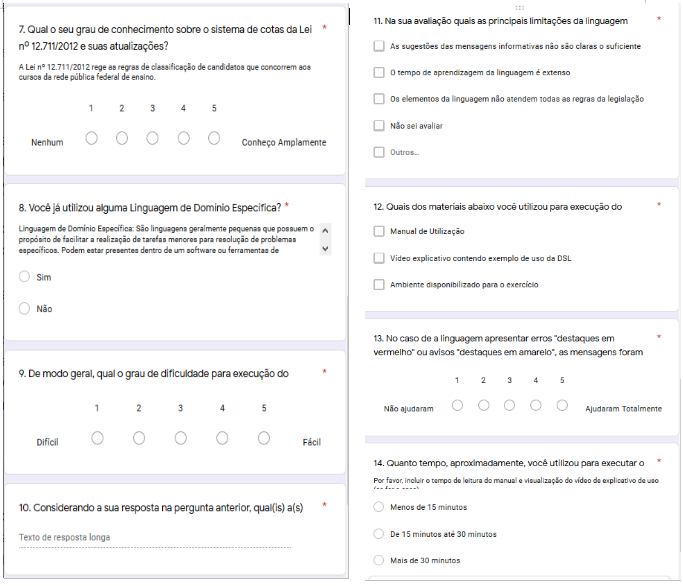
\includegraphics[width=1.00\textwidth]{chapters/metodologia/imagens/questionario2.png}}

\par\medskip\textbf{Fonte:} Elaborada pelo autor (2020). \par\medskip

\end{figure}

 
 \newpage
 Na sequência, a Seção \ref{metodoapi} descreve os procedimentos metodológicos criados de modo a possibilitar a avaliação da \gls{API}.
 

\subsection{Metodologia de avaliação da API}
\label{metodoapi}
Tendo como base a DSL elaborada, uma \gls{API} foi desenvolvida para disponibilizar \textit{endpoints} responsáveis pelos métodos de classificação e de aprovação de candidatos. Para tanto, as regras definidas na linguagem foram exportadas em formato de arquivos JSON, os quais foram utilizados no framework \textit{SpringBoot} \footnote{Segundo \citeonline{springbootreference}, o Spring Boot é um projeto da Spring que visa simplificar a criação de aplicações Java com base no Spring \textit{Framework}, para que se tenha uma aplicação inicial sem a necessidade de muitas configurações.} para geração das operações \gls{API}. 

Desse modo, foi possível executar a classificação dos candidatos e fazer a comparação com os resultados de 13494 candidatos presentes na base de dados do sistema de ingresso. No total 16 processos foram selecionados aleatoriamente entre as diferentes versões de lei nas quais foram realizadas classificações pelas regras de cotas, conforme mencionado e apresentado na Figura \ref{processos_utilizados}. Para documentar as divergências entre os resultados da \gls{API} e do histórico presente no banco de dados do sistema utilizou-se o recurso de \textit{issues} disponível no sistema de controle de versão \textit{github} (Figura \ref{fig:issues}). Para cada curso com diferenças nas situações de classificações foi descrita a versão de lei aplicada na classificação, a quantidade de vagas, o problema apresentado, o motivo encontrado e uma possível solução.

\begin{figure}[ht!]
\centering

\caption{\textmd{Issues da \gls{API} no GitHub}}
\label{fig:issues}
\fcolorbox{gray}{white}{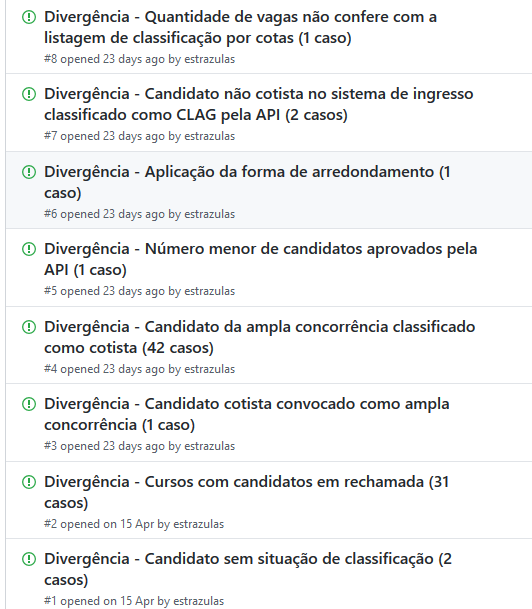
\includegraphics[width=0.70\textwidth]{chapters/metodologia/imagens/issues.png}}

\par\medskip\textbf{Fonte:} Elaborada pelo autor (2020). \par\medskip

\end{figure}



O detalhamento completo de implementação da \gls{API} foi descrito no Capítulo \ref{chap:dslcotas} e a análise das divergências encontradas está presente no Capítulo \ref{chap:analise}. Por fim, no próximo Capítulo estão presentes os principais conceitos encontrados na literatura que serviram como base para fundamentar o desenvolvimento dessa pesquisa.